\begin{figure}[!h]
  \centerline{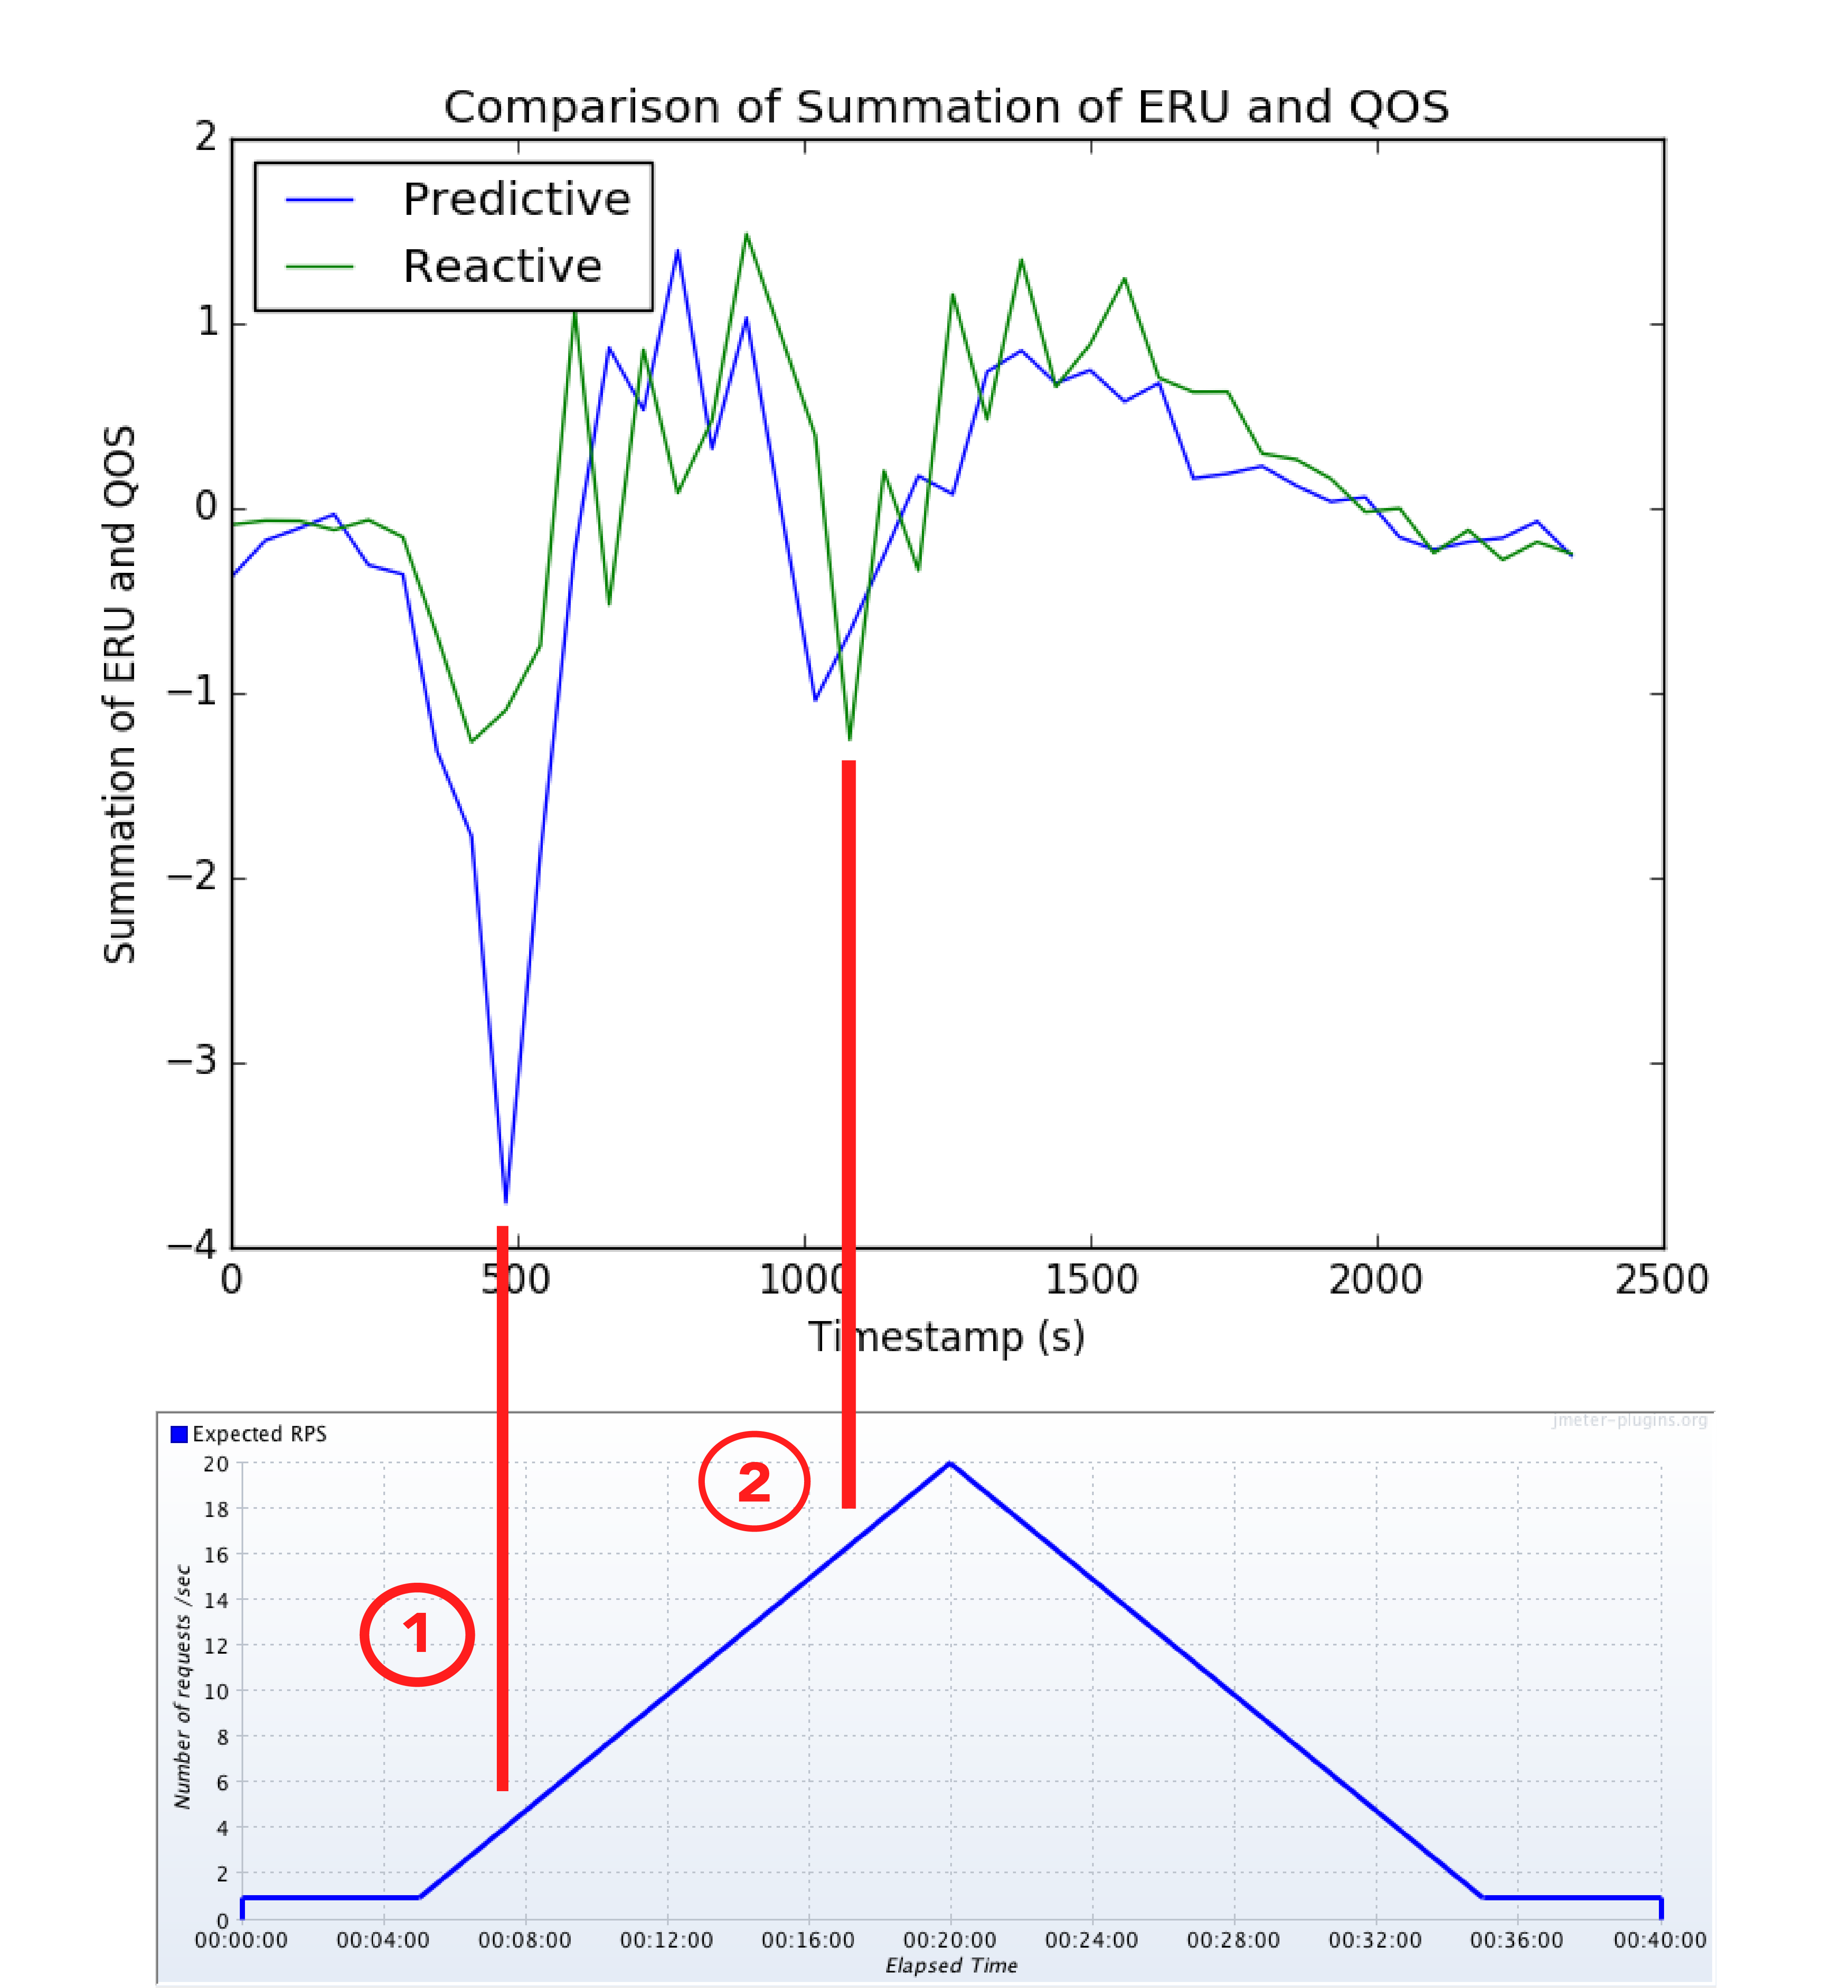
\includegraphics[scale=.70]{increase-decrease-labelled.png}}
  \caption{A comparison of the summation of ERU and QoS for
    predictive and reactive auto-scaling for 135s, increase-decrease}
  \label{fig:135s-increase-decrease-labelled}
\end{figure}

Figure \ref{fig:135s-increase-decrease-labelled} contains a graph
showing predictive and reactive auto-scaling's different
summations of efficient resource utilization and quality of service over the
course of the \textit{increase-decrease} trial. In contrast to our previous two
traffic patterns, we find that predictive auto-scaling is not particularly
beneficial in this context. Specifically, if we look at the moment labelled
$1$ on \ref{fig:135s-increase-decrease-labelled}, we an instance in which
predictive auto-scaling suffers a severe performance decrease in comparison to
reactive auto-scaling. We trace this decrease again to under-provsioning. In
this scenario, the introductory buffer period has caused our linear prediction
algorithm to underestimate the slope of the line indicating the rise in load. As
such, the reactive auto-scaling algorithm actually has a more aggressive opinion
of the load the application will face. As this aggressive understanding is
confirmed by our actual increase, reactive auto-scaling outperforms predictive
auto-scaling on the \textit{increase-decrease} traffic-pattern.

\begin{table}[htbp]
  \centering
  \caption{Difference in Predictive and Reactive Auto-scaling for 135s, increase-decrease}
  \label{tab:135s-increase-decrease}
\begin{tabular}{l c}\hline\hline
    \multicolumn{1}{c}{\textbf{Measure}} & \textbf{Value} \\ \hline
     p-value & 0.638 \\
     z-score & -.0352 \\
     std\_dev & 0.680 \\
     mean & -0.234
  \end{tabular}
\end{table}

Figure \ref{fig:135s-increase-decrease-labelled} shows that predictive
auto-scaling is actually slightly detrimental on the \textit{increase-decrease} traffic pattern,
Still, Table \ref{tab:135s-increase-decrease} shows that we are not able to claim
statistical significance with respect to these results, and thus should not be
too confident that prediction plays a negative effect. Rather, it appears to
have very little impact in either direction on this traffic pattern.
